\documentclass[a4paper]{book}
\usepackage{a4wide}
\usepackage{makeidx}
\usepackage{fancyhdr}
\usepackage{graphicx}
\usepackage{multicol}
\usepackage{float}
\usepackage{textcomp}
\usepackage{alltt}
\usepackage{times}
\usepackage{ifpdf}
\ifpdf
\usepackage[pdftex,
            pagebackref=true,
            colorlinks=true,
            linkcolor=blue,
            unicode
           ]{hyperref}
\else
\usepackage[ps2pdf,
            pagebackref=true,
            colorlinks=true,
            linkcolor=blue,
            unicode
           ]{hyperref}
\usepackage{pspicture}
\fi
\usepackage[utf8]{inputenc}
\usepackage{doxygen}
\makeindex
\setcounter{tocdepth}{3}
\renewcommand{\footrulewidth}{0.4pt}
\begin{document}
\begin{titlepage}
\vspace*{7cm}
\begin{center}
{\Large Platform 2D Game Engine \\[1ex]\large v0.0.1 Pre-Alpha }\\
\vspace*{1cm}
{\large Generated by Doxygen 1.5.8}\\
\vspace*{0.5cm}
{\small Thu Apr 30 00:54:34 2009}\\
\end{center}
\end{titlepage}
\clearemptydoublepage
\pagenumbering{roman}
\tableofcontents
\clearemptydoublepage
\pagenumbering{arabic}
\chapter{Class Index}
\section{Class Hierarchy}
This inheritance list is sorted roughly, but not completely, alphabetically:\begin{CompactList}
\item \contentsline{section}{Platform::GameMap}{\pageref{de/db6/class_platform_1_1_game_map}}{}
\item \contentsline{section}{Platform::GameMapLayer}{\pageref{d8/d53/class_platform_1_1_game_map_layer}}{}
\item \contentsline{section}{Platform::GamePlayer}{\pageref{d4/d4e/class_platform_1_1_game_player}}{}
\item \contentsline{section}{Platform::GameState}{\pageref{d4/d4f/class_platform_1_1_game_state}}{}
\begin{CompactList}
\item \contentsline{section}{Platform::GameStaticMovementState}{\pageref{db/d55/class_platform_1_1_game_static_movement_state}}{}
\end{CompactList}
\item \contentsline{section}{Platform::PlatformEngine}{\pageref{d2/dd5/class_platform_1_1_platform_engine}}{}
\end{CompactList}

\chapter{Class Index}
\section{Class List}
Here are the classes, structs, unions and interfaces with brief descriptions:\begin{CompactList}
\item\contentsline{section}{\hyperlink{class_game_map}{GameMap} (The map being used by the navigation state )}{\pageref{class_game_map}}{}
\item\contentsline{section}{\hyperlink{class_game_map_layer}{GameMapLayer} (A section of the map object )}{\pageref{class_game_map_layer}}{}
\item\contentsline{section}{\hyperlink{class_game_navigation_state}{GameNavigationState} (The state in which game world navigation takes place )}{\pageref{class_game_navigation_state}}{}
\item\contentsline{section}{\hyperlink{class_game_state}{GameState} (A state of behavior for the engine )}{\pageref{class_game_state}}{}
\item\contentsline{section}{\hyperlink{class_platform_engine}{PlatformEngine} (The game engine instance )}{\pageref{class_platform_engine}}{}
\end{CompactList}

\chapter{Class Documentation}
\hypertarget{class_game_map}{
\section{GameMap Class Reference}
\label{d4/de2/class_game_map}\index{GameMap@{GameMap}}
}
The map being used by the navigation state.  


{\tt \#include $<$GameMap.h$>$}

\subsection*{Public Member Functions}
\begin{CompactItemize}
\item 
\hyperlink{class_game_map_ae71e5694cf19612fcaa4c1e21b03b71}{GameMap} ()
\item 
void \hyperlink{class_game_map_e9b33ef01ca643a2389e7be0ebf838b1}{MoveMapUp} ()
\item 
void \hyperlink{class_game_map_7466202e8f2bd3ae188ddcbd7e50a023}{MoveMapDown} ()
\item 
void \hyperlink{class_game_map_90fe97ecdcee40995d8e5fa86857cf5c}{MoveMapLeft} ()
\item 
void \hyperlink{class_game_map_e76fd062e8e47331e7e999dbea0f0486}{MoveMapRight} ()
\item 
void \hyperlink{class_game_map_c289ffedd32b98d2827e6b765b3e50d6}{Draw} (\hyperlink{class_platform_engine}{PlatformEngine} $\ast$game)
\end{CompactItemize}


\subsection{Detailed Description}
The map being used by the navigation state. 

This is a 'map', or a 'world', that can be navigated and interacted with in the game navigation state. It consists of a stack of layers, which have a number of different types that can be used for different purposes. The map contains functions that specify where on the screen grid the layers it contains should be drawn, which is how it is told by the \hyperlink{class_game_navigation_state}{GameNavigationState} which direction it should move in order to give the impression that the Player is moving about in the map. 

\subsection{Constructor \& Destructor Documentation}
\hypertarget{class_game_map_ae71e5694cf19612fcaa4c1e21b03b71}{
\index{GameMap@{GameMap}!GameMap@{GameMap}}
\index{GameMap@{GameMap}!GameMap@{GameMap}}
\subsubsection[{GameMap}]{\setlength{\rightskip}{0pt plus 5cm}GameMap::GameMap ()}}
\label{d4/de2/class_game_map_ae71e5694cf19612fcaa4c1e21b03b71}




\subsection{Member Function Documentation}
\hypertarget{class_game_map_c289ffedd32b98d2827e6b765b3e50d6}{
\index{GameMap@{GameMap}!Draw@{Draw}}
\index{Draw@{Draw}!GameMap@{GameMap}}
\subsubsection[{Draw}]{\setlength{\rightskip}{0pt plus 5cm}void GameMap::Draw ({\bf PlatformEngine} $\ast$ {\em game})}}
\label{d4/de2/class_game_map_c289ffedd32b98d2827e6b765b3e50d6}


\hypertarget{class_game_map_7466202e8f2bd3ae188ddcbd7e50a023}{
\index{GameMap@{GameMap}!MoveMapDown@{MoveMapDown}}
\index{MoveMapDown@{MoveMapDown}!GameMap@{GameMap}}
\subsubsection[{MoveMapDown}]{\setlength{\rightskip}{0pt plus 5cm}void GameMap::MoveMapDown ()}}
\label{d4/de2/class_game_map_7466202e8f2bd3ae188ddcbd7e50a023}


\hypertarget{class_game_map_90fe97ecdcee40995d8e5fa86857cf5c}{
\index{GameMap@{GameMap}!MoveMapLeft@{MoveMapLeft}}
\index{MoveMapLeft@{MoveMapLeft}!GameMap@{GameMap}}
\subsubsection[{MoveMapLeft}]{\setlength{\rightskip}{0pt plus 5cm}void GameMap::MoveMapLeft ()}}
\label{d4/de2/class_game_map_90fe97ecdcee40995d8e5fa86857cf5c}


\hypertarget{class_game_map_e76fd062e8e47331e7e999dbea0f0486}{
\index{GameMap@{GameMap}!MoveMapRight@{MoveMapRight}}
\index{MoveMapRight@{MoveMapRight}!GameMap@{GameMap}}
\subsubsection[{MoveMapRight}]{\setlength{\rightskip}{0pt plus 5cm}void GameMap::MoveMapRight ()}}
\label{d4/de2/class_game_map_e76fd062e8e47331e7e999dbea0f0486}


\hypertarget{class_game_map_e9b33ef01ca643a2389e7be0ebf838b1}{
\index{GameMap@{GameMap}!MoveMapUp@{MoveMapUp}}
\index{MoveMapUp@{MoveMapUp}!GameMap@{GameMap}}
\subsubsection[{MoveMapUp}]{\setlength{\rightskip}{0pt plus 5cm}void GameMap::MoveMapUp ()}}
\label{d4/de2/class_game_map_e9b33ef01ca643a2389e7be0ebf838b1}



\hypertarget{class_game_map_layer}{
\section{GameMapLayer Class Reference}
\label{d2/d95/class_game_map_layer}\index{GameMapLayer@{GameMapLayer}}
}
A section of the map object.  


{\tt \#include $<$GameMapLayer.h$>$}

\subsection*{Public Member Functions}
\begin{CompactItemize}
\item 
\hyperlink{class_game_map_layer_92a1d055fbbf7f7c2d974038596b857e}{GameMapLayer} ()
\item 
virtual void \hyperlink{class_game_map_layer_d82f8be1c403ce3e55d5ed9177aad68c}{Draw} (SDL\_\-Surface $\ast$mainScreen)=0
\end{CompactItemize}


\subsection{Detailed Description}
A section of the map object. 

This is an abstract class representing a layer of the map object used by the Navigation State. It is not meant to be used, but is the ancestor of several specific types of map layers. 

\subsection{Constructor \& Destructor Documentation}
\hypertarget{class_game_map_layer_92a1d055fbbf7f7c2d974038596b857e}{
\index{GameMapLayer@{GameMapLayer}!GameMapLayer@{GameMapLayer}}
\index{GameMapLayer@{GameMapLayer}!GameMapLayer@{GameMapLayer}}
\subsubsection[{GameMapLayer}]{\setlength{\rightskip}{0pt plus 5cm}GameMapLayer::GameMapLayer ()}}
\label{d2/d95/class_game_map_layer_92a1d055fbbf7f7c2d974038596b857e}




\subsection{Member Function Documentation}
\hypertarget{class_game_map_layer_d82f8be1c403ce3e55d5ed9177aad68c}{
\index{GameMapLayer@{GameMapLayer}!Draw@{Draw}}
\index{Draw@{Draw}!GameMapLayer@{GameMapLayer}}
\subsubsection[{Draw}]{\setlength{\rightskip}{0pt plus 5cm}virtual void GameMapLayer::Draw (SDL\_\-Surface $\ast$ {\em mainScreen})\hspace{0.3cm}{\tt  \mbox{[}pure virtual\mbox{]}}}}
\label{d2/d95/class_game_map_layer_d82f8be1c403ce3e55d5ed9177aad68c}



\hypertarget{class_game_player}{
\section{GamePlayer Class Reference}
\label{d7/df6/class_game_player}\index{GamePlayer@{GamePlayer}}
}
The player character entity.  


{\tt \#include $<$GamePlayer.h$>$}

\subsection*{Public Member Functions}
\begin{CompactItemize}
\item 
\hyperlink{class_game_player_f0314668e232831d2f9c263596dccde6}{GamePlayer} ()
\item 
void \hyperlink{class_game_player_61b39fe229f10d4f93d4eb96754a2961}{Init} ()
\item 
void \hyperlink{class_game_player_3394352e57e918eb17fec46498f5e348}{DrawPlayer} (\hyperlink{class_platform_engine}{PlatformEngine} $\ast$game)
\item 
void \hyperlink{class_game_player_46aa70e41a260b0ea8afdae38052d65c}{MovePlayer} (SDL\_\-Rect \&delta)
\end{CompactItemize}


\subsection{Detailed Description}
The player character entity. 

\hyperlink{class_game_player}{GamePlayer} is an entity representing the avatar of the human player on the screen. It is usually the center focus of the player's attention and the proxy through which the player expects to operate. 

\subsection{Constructor \& Destructor Documentation}
\hypertarget{class_game_player_f0314668e232831d2f9c263596dccde6}{
\index{GamePlayer@{GamePlayer}!GamePlayer@{GamePlayer}}
\index{GamePlayer@{GamePlayer}!GamePlayer@{GamePlayer}}
\subsubsection[{GamePlayer}]{\setlength{\rightskip}{0pt plus 5cm}GamePlayer::GamePlayer ()}}
\label{d7/df6/class_game_player_f0314668e232831d2f9c263596dccde6}




\subsection{Member Function Documentation}
\hypertarget{class_game_player_3394352e57e918eb17fec46498f5e348}{
\index{GamePlayer@{GamePlayer}!DrawPlayer@{DrawPlayer}}
\index{DrawPlayer@{DrawPlayer}!GamePlayer@{GamePlayer}}
\subsubsection[{DrawPlayer}]{\setlength{\rightskip}{0pt plus 5cm}void GamePlayer::DrawPlayer ({\bf PlatformEngine} $\ast$ {\em game})}}
\label{d7/df6/class_game_player_3394352e57e918eb17fec46498f5e348}


\hypertarget{class_game_player_61b39fe229f10d4f93d4eb96754a2961}{
\index{GamePlayer@{GamePlayer}!Init@{Init}}
\index{Init@{Init}!GamePlayer@{GamePlayer}}
\subsubsection[{Init}]{\setlength{\rightskip}{0pt plus 5cm}void GamePlayer::Init ()}}
\label{d7/df6/class_game_player_61b39fe229f10d4f93d4eb96754a2961}


\hypertarget{class_game_player_46aa70e41a260b0ea8afdae38052d65c}{
\index{GamePlayer@{GamePlayer}!MovePlayer@{MovePlayer}}
\index{MovePlayer@{MovePlayer}!GamePlayer@{GamePlayer}}
\subsubsection[{MovePlayer}]{\setlength{\rightskip}{0pt plus 5cm}void GamePlayer::MovePlayer (SDL\_\-Rect \& {\em delta})}}
\label{d7/df6/class_game_player_46aa70e41a260b0ea8afdae38052d65c}



\hypertarget{class_game_state}{
\section{GameState Class Reference}
\label{class_game_state}\index{GameState@{GameState}}
}
A state of behavior for the engine.  


{\tt \#include $<$GameState.h$>$}

Inheritance diagram for GameState::\begin{figure}[H]
\begin{center}
\leavevmode
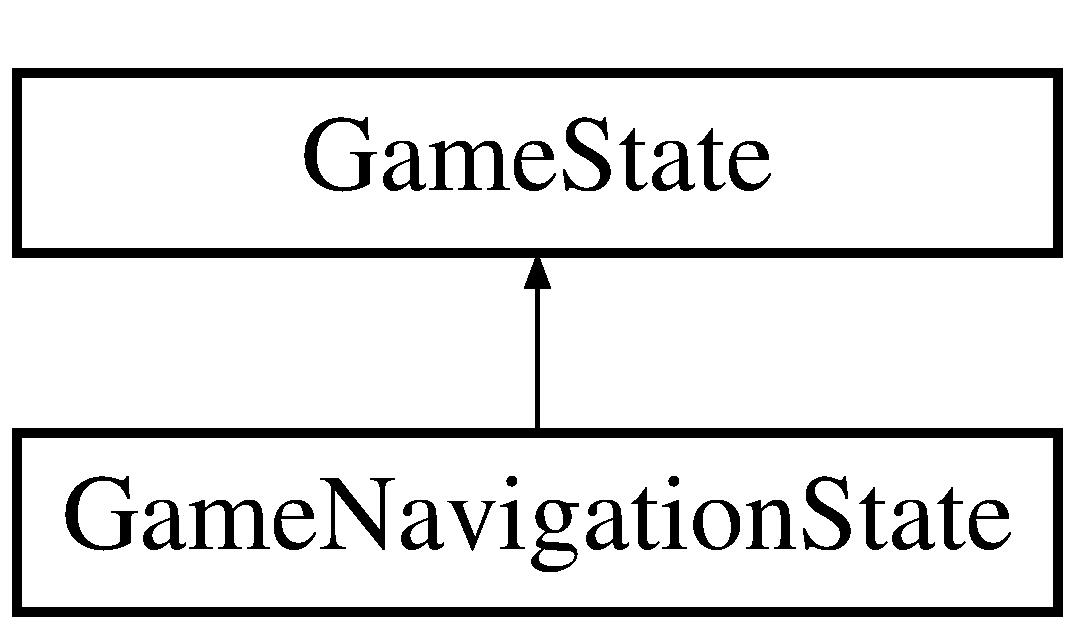
\includegraphics[height=2cm]{class_game_state}
\end{center}
\end{figure}
\subsection*{Public Member Functions}
\begin{CompactItemize}
\item 
\hyperlink{class_game_state_4fa0a2bf50315c4a35a3890a0adcee5c}{GameState} ()
\item 
virtual void \hyperlink{class_game_state_eec488593bae214c0f738bd64dafba32}{Init} ()=0
\item 
virtual void \hyperlink{class_game_state_041e7a5430d71da84745af11abdacd93}{Cleanup} ()=0
\item 
virtual void \hyperlink{class_game_state_1f4d2b5a2e4dcb7645e3e7a5735926a6}{Pause} ()=0
\item 
virtual void \hyperlink{class_game_state_cf9bcd5b47ebb3f572389f64c5ca5ed4}{Resume} ()=0
\item 
virtual void \hyperlink{class_game_state_82a31f1480fc637829d6630c01570d4c}{HandleEvents} (\hyperlink{class_platform_engine}{PlatformEngine} $\ast$game, SDL\_\-Event \&event)=0
\item 
virtual void \hyperlink{class_game_state_100ca49bc95afce1d5c5b756708bbc2b}{Update} (\hyperlink{class_platform_engine}{PlatformEngine} $\ast$game)=0
\item 
virtual void \hyperlink{class_game_state_7333dda0f49b3fa1c01cd3295f853024}{Draw} (\hyperlink{class_platform_engine}{PlatformEngine} $\ast$game)=0
\item 
void \hyperlink{class_game_state_f786aeb704a22a135dc289bb89fcc452}{ChangeState} (\hyperlink{class_platform_engine}{PlatformEngine} $\ast$game, \hyperlink{class_game_state}{GameState} $\ast$state)
\end{CompactItemize}


\subsection{Detailed Description}
A state of behavior for the engine. 

A Game State is a layer on top of the default engine behavior that requires a custom form of behavior for its operation. In the Platform engine, the an instance of the engine stores the current state on a stack, and any newly initiated states can be placed on top of the stack. The normal engine functions will generally call the corresponding operation functions from the state at the top of the stack, so that the engine's operation is ultimately controlled by the current top state.

This class in particular is an abstract class, not intended for actual use. The derivative classes, which are the different kinds of states, are used in normal program operations. 

\subsection{Constructor \& Destructor Documentation}
\hypertarget{class_game_state_4fa0a2bf50315c4a35a3890a0adcee5c}{
\index{GameState@{GameState}!GameState@{GameState}}
\index{GameState@{GameState}!GameState@{GameState}}
\subsubsection[{GameState}]{\setlength{\rightskip}{0pt plus 5cm}GameState::GameState ()}}
\label{class_game_state_4fa0a2bf50315c4a35a3890a0adcee5c}




\subsection{Member Function Documentation}
\hypertarget{class_game_state_f786aeb704a22a135dc289bb89fcc452}{
\index{GameState@{GameState}!ChangeState@{ChangeState}}
\index{ChangeState@{ChangeState}!GameState@{GameState}}
\subsubsection[{ChangeState}]{\setlength{\rightskip}{0pt plus 5cm}void GameState::ChangeState ({\bf PlatformEngine} $\ast$ {\em game}, \/  {\bf GameState} $\ast$ {\em state})\hspace{0.3cm}{\tt  \mbox{[}inline\mbox{]}}}}
\label{class_game_state_f786aeb704a22a135dc289bb89fcc452}


\hypertarget{class_game_state_041e7a5430d71da84745af11abdacd93}{
\index{GameState@{GameState}!Cleanup@{Cleanup}}
\index{Cleanup@{Cleanup}!GameState@{GameState}}
\subsubsection[{Cleanup}]{\setlength{\rightskip}{0pt plus 5cm}virtual void GameState::Cleanup ()\hspace{0.3cm}{\tt  \mbox{[}pure virtual\mbox{]}}}}
\label{class_game_state_041e7a5430d71da84745af11abdacd93}




Implemented in \hyperlink{class_game_navigation_state_f93a7dbb7eac4b14a6d59cbca32b9abd}{GameNavigationState}.\hypertarget{class_game_state_7333dda0f49b3fa1c01cd3295f853024}{
\index{GameState@{GameState}!Draw@{Draw}}
\index{Draw@{Draw}!GameState@{GameState}}
\subsubsection[{Draw}]{\setlength{\rightskip}{0pt plus 5cm}virtual void GameState::Draw ({\bf PlatformEngine} $\ast$ {\em game})\hspace{0.3cm}{\tt  \mbox{[}pure virtual\mbox{]}}}}
\label{class_game_state_7333dda0f49b3fa1c01cd3295f853024}




Implemented in \hyperlink{class_game_navigation_state_a37dce070a906454c512192c067fda09}{GameNavigationState}.\hypertarget{class_game_state_82a31f1480fc637829d6630c01570d4c}{
\index{GameState@{GameState}!HandleEvents@{HandleEvents}}
\index{HandleEvents@{HandleEvents}!GameState@{GameState}}
\subsubsection[{HandleEvents}]{\setlength{\rightskip}{0pt plus 5cm}virtual void GameState::HandleEvents ({\bf PlatformEngine} $\ast$ {\em game}, \/  SDL\_\-Event \& {\em event})\hspace{0.3cm}{\tt  \mbox{[}pure virtual\mbox{]}}}}
\label{class_game_state_82a31f1480fc637829d6630c01570d4c}




Implemented in \hyperlink{class_game_navigation_state_c47e8f7b8802e7b7e7b5076c20313596}{GameNavigationState}.\hypertarget{class_game_state_eec488593bae214c0f738bd64dafba32}{
\index{GameState@{GameState}!Init@{Init}}
\index{Init@{Init}!GameState@{GameState}}
\subsubsection[{Init}]{\setlength{\rightskip}{0pt plus 5cm}virtual void GameState::Init ()\hspace{0.3cm}{\tt  \mbox{[}pure virtual\mbox{]}}}}
\label{class_game_state_eec488593bae214c0f738bd64dafba32}




Implemented in \hyperlink{class_game_navigation_state_8f613860bf544476ab9cff9fb7f98201}{GameNavigationState}.\hypertarget{class_game_state_1f4d2b5a2e4dcb7645e3e7a5735926a6}{
\index{GameState@{GameState}!Pause@{Pause}}
\index{Pause@{Pause}!GameState@{GameState}}
\subsubsection[{Pause}]{\setlength{\rightskip}{0pt plus 5cm}virtual void GameState::Pause ()\hspace{0.3cm}{\tt  \mbox{[}pure virtual\mbox{]}}}}
\label{class_game_state_1f4d2b5a2e4dcb7645e3e7a5735926a6}




Implemented in \hyperlink{class_game_navigation_state_ac626b511de8af9f32b7a1492a10f861}{GameNavigationState}.\hypertarget{class_game_state_cf9bcd5b47ebb3f572389f64c5ca5ed4}{
\index{GameState@{GameState}!Resume@{Resume}}
\index{Resume@{Resume}!GameState@{GameState}}
\subsubsection[{Resume}]{\setlength{\rightskip}{0pt plus 5cm}virtual void GameState::Resume ()\hspace{0.3cm}{\tt  \mbox{[}pure virtual\mbox{]}}}}
\label{class_game_state_cf9bcd5b47ebb3f572389f64c5ca5ed4}




Implemented in \hyperlink{class_game_navigation_state_4d6aee55eddb1978f493206d985fb950}{GameNavigationState}.\hypertarget{class_game_state_100ca49bc95afce1d5c5b756708bbc2b}{
\index{GameState@{GameState}!Update@{Update}}
\index{Update@{Update}!GameState@{GameState}}
\subsubsection[{Update}]{\setlength{\rightskip}{0pt plus 5cm}virtual void GameState::Update ({\bf PlatformEngine} $\ast$ {\em game})\hspace{0.3cm}{\tt  \mbox{[}pure virtual\mbox{]}}}}
\label{class_game_state_100ca49bc95afce1d5c5b756708bbc2b}




Implemented in \hyperlink{class_game_navigation_state_90f5e6d6287a875d8f2737180f46a004}{GameNavigationState}.
\hypertarget{class_game_static_movement_state}{
\section{GameStaticMovementState Class Reference}
\label{d7/d3b/class_game_static_movement_state}\index{GameStaticMovementState@{GameStaticMovementState}}
}
A state where entities move on a static playfield.  


{\tt \#include $<$GameStaticMovementState.h$>$}

Inheritance diagram for GameStaticMovementState:\nopagebreak
\begin{figure}[H]
\begin{center}
\leavevmode
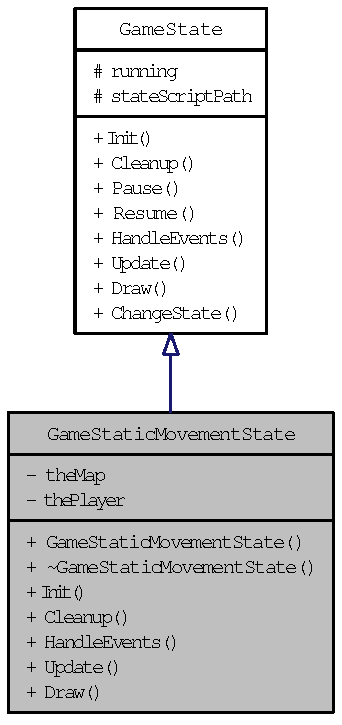
\includegraphics[width=200pt]{d0/d7e/class_game_static_movement_state__inherit__graph}
\end{center}
\end{figure}
Collaboration diagram for GameStaticMovementState:\nopagebreak
\begin{figure}[H]
\begin{center}
\leavevmode
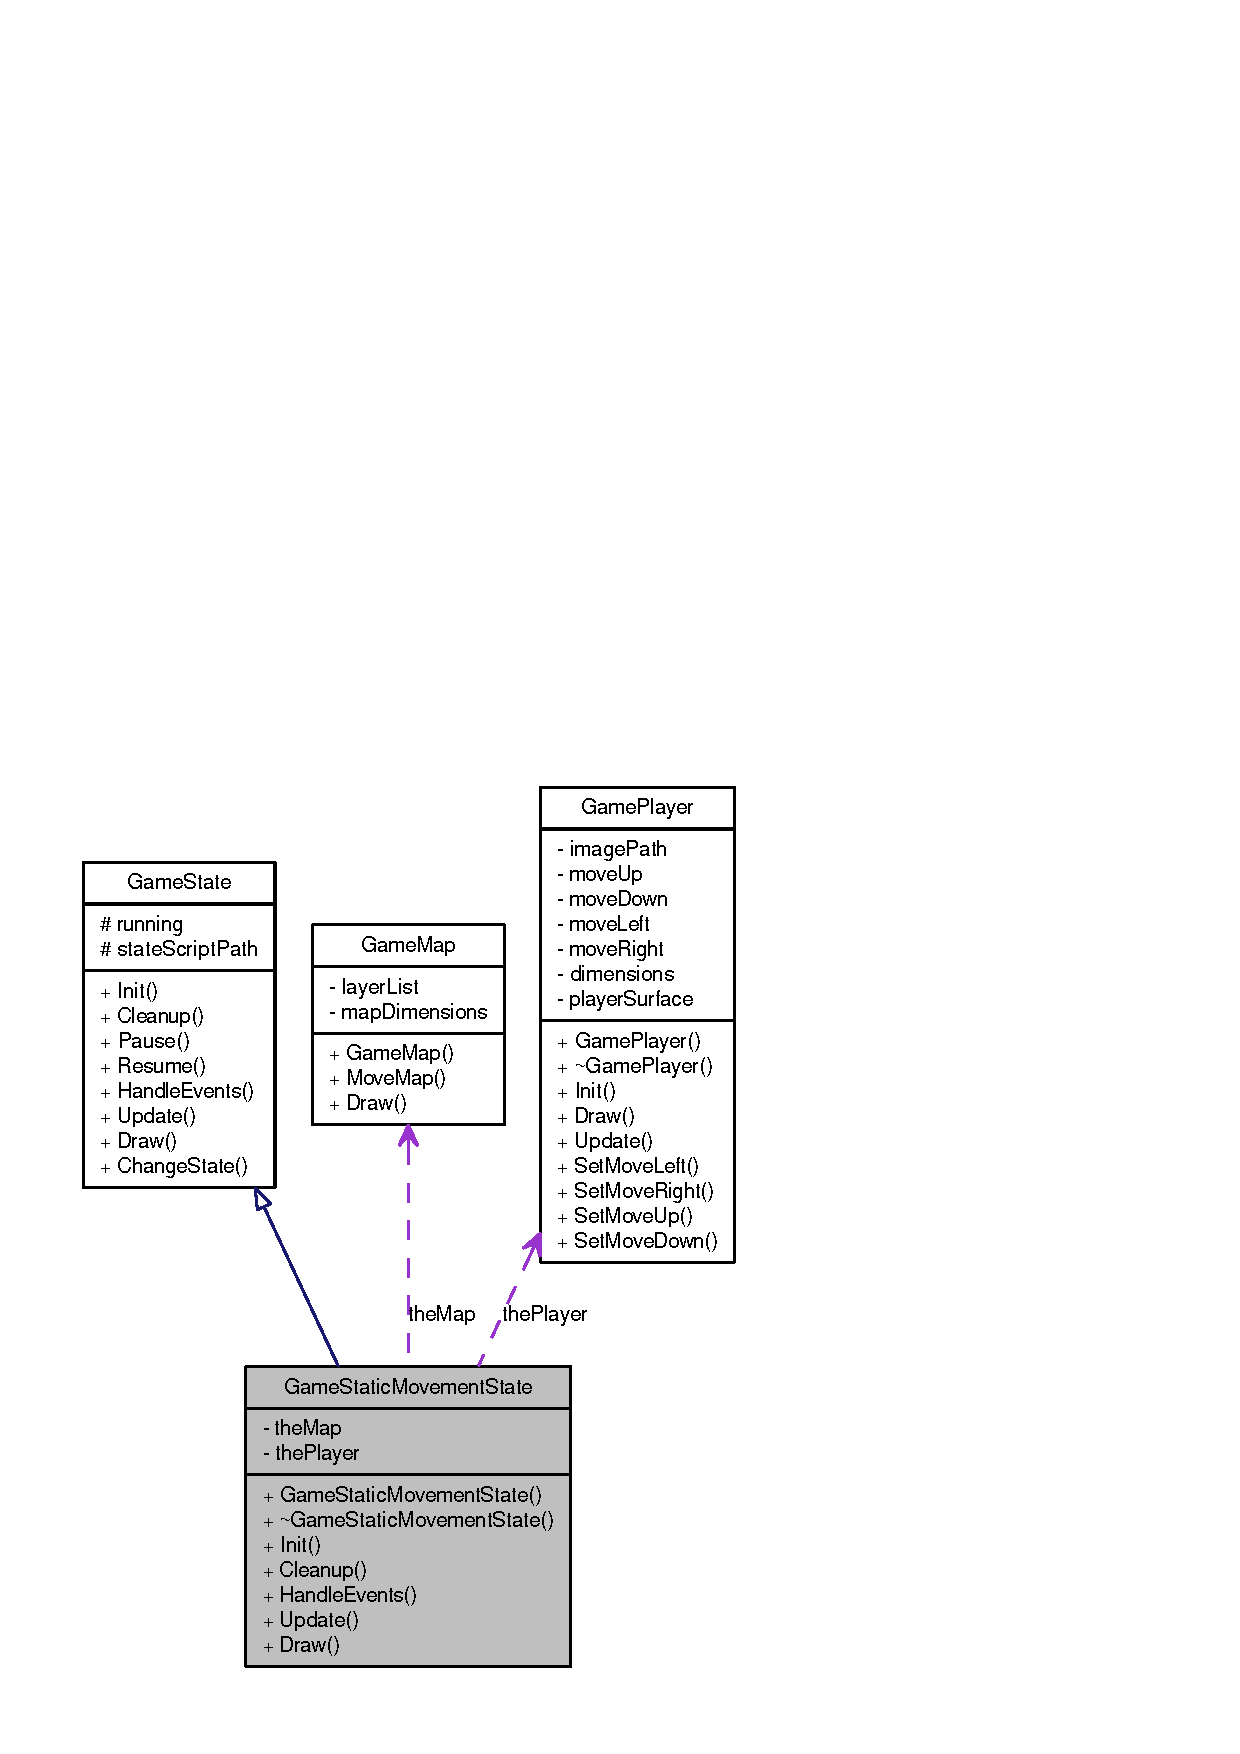
\includegraphics[height=400pt]{d3/d3d/class_game_static_movement_state__coll__graph}
\end{center}
\end{figure}
\subsection*{Public Member Functions}
\begin{CompactItemize}
\item 
\hyperlink{class_game_static_movement_state_13354d331108d7aeb78822e629d631b3}{GameStaticMovementState} ()
\item 
\hyperlink{class_game_static_movement_state_3b89c6650fba993b81abd1d5b11a82c3}{$\sim$GameStaticMovementState} ()
\item 
void \hyperlink{class_game_static_movement_state_4cb4be5ea96a6bb7b06c79bed64c355d}{Init} (const char $\ast$theScript=NULL)
\item 
void \hyperlink{class_game_static_movement_state_072662abaf5a872f7919e7fc44200a04}{Cleanup} ()
\item 
bool \hyperlink{class_game_static_movement_state_c73d6f93fee2ac6cb2788eb2984bb305}{HandleEvents} (\hyperlink{class_platform_engine}{PlatformEngine} $\ast$game, SDL\_\-Event \&event)
\item 
void \hyperlink{class_game_static_movement_state_5a3bd910a85487be371c088a1be16996}{Update} (\hyperlink{class_platform_engine}{PlatformEngine} $\ast$game)
\item 
void \hyperlink{class_game_static_movement_state_2c2d82b3dbc8e431682b53ce05294f27}{Draw} (SDL\_\-Surface $\ast$mainScreen)
\item 
virtual void \hyperlink{class_game_state_0c47c6969a4e0bb32d6cdf7bf9376817}{Pause} ()
\item 
virtual void \hyperlink{class_game_state_d12ece3c3fb066281b73b07a315f04e8}{Resume} ()
\item 
void \hyperlink{class_game_state_f786aeb704a22a135dc289bb89fcc452}{ChangeState} (\hyperlink{class_platform_engine}{PlatformEngine} $\ast$game, \hyperlink{class_game_state}{GameState} $\ast$state)
\end{CompactItemize}
\subsection*{Protected Attributes}
\begin{CompactItemize}
\item 
bool \hyperlink{class_game_state_391df04a740c7480270d3c71a578b43a}{running}
\item 
char $\ast$ \hyperlink{class_game_state_bfe09abe78dd5794426964d3392b2973}{stateScriptPath}
\end{CompactItemize}


\subsection{Detailed Description}
A state where entities move on a static playfield. 

Static Movement refers to the idea that, while there are entities moving around on the \char`\"{}map\char`\"{} area, the area itself is no larger than the size of the player's screen, and therefore doesn't move at all; in other words, it is \char`\"{}static\char`\"{}.

Note that this doesn't mean that the background can't give the illusion of movement. For example, the background might be an image that constantly scrolls downward, acting as a parallax background. However, as far as the state is concerned, the activities in the background are irrelevant; the only activity the state is concerned with is that of the entities known to it, such as the player. 

\subsection{Constructor \& Destructor Documentation}
\hypertarget{class_game_static_movement_state_13354d331108d7aeb78822e629d631b3}{
\index{GameStaticMovementState@{GameStaticMovementState}!GameStaticMovementState@{GameStaticMovementState}}
\index{GameStaticMovementState@{GameStaticMovementState}!GameStaticMovementState@{GameStaticMovementState}}
\subsubsection[{GameStaticMovementState}]{\setlength{\rightskip}{0pt plus 5cm}GameStaticMovementState::GameStaticMovementState ()}}
\label{d7/d3b/class_game_static_movement_state_13354d331108d7aeb78822e629d631b3}


\hypertarget{class_game_static_movement_state_3b89c6650fba993b81abd1d5b11a82c3}{
\index{GameStaticMovementState@{GameStaticMovementState}!$\sim$GameStaticMovementState@{$\sim$GameStaticMovementState}}
\index{$\sim$GameStaticMovementState@{$\sim$GameStaticMovementState}!GameStaticMovementState@{GameStaticMovementState}}
\subsubsection[{$\sim$GameStaticMovementState}]{\setlength{\rightskip}{0pt plus 5cm}GameStaticMovementState::$\sim$GameStaticMovementState ()}}
\label{d7/d3b/class_game_static_movement_state_3b89c6650fba993b81abd1d5b11a82c3}




\subsection{Member Function Documentation}
\hypertarget{class_game_state_f786aeb704a22a135dc289bb89fcc452}{
\index{GameStaticMovementState@{GameStaticMovementState}!ChangeState@{ChangeState}}
\index{ChangeState@{ChangeState}!GameStaticMovementState@{GameStaticMovementState}}
\subsubsection[{ChangeState}]{\setlength{\rightskip}{0pt plus 5cm}void GameState::ChangeState ({\bf PlatformEngine} $\ast$ {\em game}, \/  {\bf GameState} $\ast$ {\em state})\hspace{0.3cm}{\tt  \mbox{[}inline, inherited\mbox{]}}}}
\label{dd/d87/class_game_state_f786aeb704a22a135dc289bb89fcc452}


\hypertarget{class_game_static_movement_state_072662abaf5a872f7919e7fc44200a04}{
\index{GameStaticMovementState@{GameStaticMovementState}!Cleanup@{Cleanup}}
\index{Cleanup@{Cleanup}!GameStaticMovementState@{GameStaticMovementState}}
\subsubsection[{Cleanup}]{\setlength{\rightskip}{0pt plus 5cm}void GameStaticMovementState::Cleanup ()\hspace{0.3cm}{\tt  \mbox{[}virtual\mbox{]}}}}
\label{d7/d3b/class_game_static_movement_state_072662abaf5a872f7919e7fc44200a04}


For mostly memory management-related purposes, this will remove any assets remaining in the state.

This function is automatically called upon deletion of the state it is a member of. Thus, unless you are using the state in a nonstandard way, it should never be necessary to explicitly call this function.

\begin{Desc}
\item[Parameters:]
\begin{description}
\item[{\em theScript}]A path to the lua script that configures the initialization. \end{description}
\end{Desc}


Implements \hyperlink{class_game_state_041e7a5430d71da84745af11abdacd93}{GameState}.\hypertarget{class_game_static_movement_state_2c2d82b3dbc8e431682b53ce05294f27}{
\index{GameStaticMovementState@{GameStaticMovementState}!Draw@{Draw}}
\index{Draw@{Draw}!GameStaticMovementState@{GameStaticMovementState}}
\subsubsection[{Draw}]{\setlength{\rightskip}{0pt plus 5cm}void GameStaticMovementState::Draw (SDL\_\-Surface $\ast$ {\em mainScreen})\hspace{0.3cm}{\tt  \mbox{[}virtual\mbox{]}}}}
\label{d7/d3b/class_game_static_movement_state_2c2d82b3dbc8e431682b53ce05294f27}


This will draw any of the visible entities being used by this state to the primary display screen.

\begin{Desc}
\item[Parameters:]
\begin{description}
\item[{\em mainScreen}]A pointer to the primary display screen. \end{description}
\end{Desc}


Implements \hyperlink{class_game_state_1b93233932defca939eed4c0676a5d2a}{GameState}.\hypertarget{class_game_static_movement_state_c73d6f93fee2ac6cb2788eb2984bb305}{
\index{GameStaticMovementState@{GameStaticMovementState}!HandleEvents@{HandleEvents}}
\index{HandleEvents@{HandleEvents}!GameStaticMovementState@{GameStaticMovementState}}
\subsubsection[{HandleEvents}]{\setlength{\rightskip}{0pt plus 5cm}bool GameStaticMovementState::HandleEvents ({\bf PlatformEngine} $\ast$ {\em game}, \/  SDL\_\-Event \& {\em event})\hspace{0.3cm}{\tt  \mbox{[}virtual\mbox{]}}}}
\label{d7/d3b/class_game_static_movement_state_c73d6f93fee2ac6cb2788eb2984bb305}


Handles the events used by the state. An event that was previously polled by the engine is analyzed by this function to execute the appropriate action for that event.

\begin{Desc}
\item[Parameters:]
\begin{description}
\item[{\em game}]A pointer to the game engine. \item[{\em event}]The event that is being analyzed. \end{description}
\end{Desc}


Implements \hyperlink{class_game_state_de7bd9bda91253614322ca0ea77b7a14}{GameState}.\hypertarget{class_game_static_movement_state_4cb4be5ea96a6bb7b06c79bed64c355d}{
\index{GameStaticMovementState@{GameStaticMovementState}!Init@{Init}}
\index{Init@{Init}!GameStaticMovementState@{GameStaticMovementState}}
\subsubsection[{Init}]{\setlength{\rightskip}{0pt plus 5cm}void GameStaticMovementState::Init (const char $\ast$ {\em theScript} = {\tt NULL})\hspace{0.3cm}{\tt  \mbox{[}virtual\mbox{]}}}}
\label{d7/d3b/class_game_static_movement_state_4cb4be5ea96a6bb7b06c79bed64c355d}


The state is not initialized automatically when it is created. In order for the state to operate in any realistic way, it must be initialized with this function, along with a lua script giving the details of its operation.

\begin{Desc}
\item[Parameters:]
\begin{description}
\item[{\em theScript}]A path to the lua script that configures the initialization. \end{description}
\end{Desc}


First, the engine removes the paths of any previous scripts, assuming they exist, before loading the script that has been passed to it.

The state then loads a lua interpreter to read the script file. If no script is passed, then the function will only mark the state as \char`\"{}running\char`\"{}, while effectively having no assets defined.

The function loads the variable \char`\"{}playerImage\char`\"{} from the script, and then retains the path of the image as a string.

A new \hyperlink{class_game_player}{GamePlayer} entity is then created, and it is initialized using the image that was loaded from the script.

The state is then set as \char`\"{}running\char`\"{} so that normal operation can begin.

Implements \hyperlink{class_game_state_488fd39ceb2907b13e11f03607f16e5f}{GameState}.\hypertarget{class_game_state_0c47c6969a4e0bb32d6cdf7bf9376817}{
\index{GameStaticMovementState@{GameStaticMovementState}!Pause@{Pause}}
\index{Pause@{Pause}!GameStaticMovementState@{GameStaticMovementState}}
\subsubsection[{Pause}]{\setlength{\rightskip}{0pt plus 5cm}void GameState::Pause ()\hspace{0.3cm}{\tt  \mbox{[}virtual, inherited\mbox{]}}}}
\label{dd/d87/class_game_state_0c47c6969a4e0bb32d6cdf7bf9376817}


Pauses the execution of this state until further notice, assuming it is currently running. If it is already paused, this has no effect. \hypertarget{class_game_state_d12ece3c3fb066281b73b07a315f04e8}{
\index{GameStaticMovementState@{GameStaticMovementState}!Resume@{Resume}}
\index{Resume@{Resume}!GameStaticMovementState@{GameStaticMovementState}}
\subsubsection[{Resume}]{\setlength{\rightskip}{0pt plus 5cm}void GameState::Resume ()\hspace{0.3cm}{\tt  \mbox{[}virtual, inherited\mbox{]}}}}
\label{dd/d87/class_game_state_d12ece3c3fb066281b73b07a315f04e8}


Resumes the execution of this state, if it has been paused previously; otherwise it has no effect. \hypertarget{class_game_static_movement_state_5a3bd910a85487be371c088a1be16996}{
\index{GameStaticMovementState@{GameStaticMovementState}!Update@{Update}}
\index{Update@{Update}!GameStaticMovementState@{GameStaticMovementState}}
\subsubsection[{Update}]{\setlength{\rightskip}{0pt plus 5cm}void GameStaticMovementState::Update ({\bf PlatformEngine} $\ast$ {\em game})\hspace{0.3cm}{\tt  \mbox{[}virtual\mbox{]}}}}
\label{d7/d3b/class_game_static_movement_state_5a3bd910a85487be371c088a1be16996}


Any calculations necessary to be regularly done for the engine logic are done.

\begin{Desc}
\item[Parameters:]
\begin{description}
\item[{\em game}]A pointer to the game engine. \end{description}
\end{Desc}


Implements \hyperlink{class_game_state_100ca49bc95afce1d5c5b756708bbc2b}{GameState}.

\subsection{Member Data Documentation}
\hypertarget{class_game_state_391df04a740c7480270d3c71a578b43a}{
\index{GameStaticMovementState@{GameStaticMovementState}!running@{running}}
\index{running@{running}!GameStaticMovementState@{GameStaticMovementState}}
\subsubsection[{running}]{\setlength{\rightskip}{0pt plus 5cm}bool {\bf GameState::running}\hspace{0.3cm}{\tt  \mbox{[}protected, inherited\mbox{]}}}}
\label{dd/d87/class_game_state_391df04a740c7480270d3c71a578b43a}


\hypertarget{class_game_state_bfe09abe78dd5794426964d3392b2973}{
\index{GameStaticMovementState@{GameStaticMovementState}!stateScriptPath@{stateScriptPath}}
\index{stateScriptPath@{stateScriptPath}!GameStaticMovementState@{GameStaticMovementState}}
\subsubsection[{stateScriptPath}]{\setlength{\rightskip}{0pt plus 5cm}char$\ast$ {\bf GameState::stateScriptPath}\hspace{0.3cm}{\tt  \mbox{[}protected, inherited\mbox{]}}}}
\label{dd/d87/class_game_state_bfe09abe78dd5794426964d3392b2973}



\hypertarget{class_platform_engine}{
\section{PlatformEngine Class Reference}
\label{class_platform_engine}\index{PlatformEngine@{PlatformEngine}}
}
The game engine instance.  


{\tt \#include $<$PlatformEngine.h$>$}

\subsection*{Public Member Functions}
\begin{CompactItemize}
\item 
\hyperlink{class_platform_engine_9d45e2da5a9b7e52d8c5636f70068e11}{PlatformEngine} ()
\item 
void \hyperlink{class_platform_engine_059814bb3f1815b15d5a892f8ea6cb4a}{Init} ()
\item 
void \hyperlink{class_platform_engine_361b54312d9ec2fa842cd982f67100f9}{Cleanup} ()
\item 
void \hyperlink{class_platform_engine_d2b335545c9ab6bce7be7c014bc8c528}{ChangeState} (\hyperlink{class_game_state}{GameState} $\ast$state)
\item 
void \hyperlink{class_platform_engine_98e3d34b6ee831bcc1d26bac83bfe8d8}{PushState} (\hyperlink{class_game_state}{GameState} $\ast$state)
\item 
void \hyperlink{class_platform_engine_cf001abec596906465197d1220db2230}{PopState} ()
\item 
void \hyperlink{class_platform_engine_7fc47bff353292f1a1435d78664df36d}{HandleEvents} ()
\item 
void \hyperlink{class_platform_engine_d3ab75304226ad3fcac6b66ce3cedbc7}{Update} ()
\item 
void \hyperlink{class_platform_engine_cd756d58f81c5e28efe98ae075367a5c}{Draw} ()
\item 
bool \hyperlink{class_platform_engine_31ec37c0222f4694cc3c0e819e143038}{Running} ()
\item 
void \hyperlink{class_platform_engine_dbcdd91813cabbe51bb2f86eb23e772a}{Quit} ()
\end{CompactItemize}


\subsection{Detailed Description}
The game engine instance. 

This class represents the game engine. It encompasses the major subprocesses; Initialization, State control, Event Handling, Updating, and Drawing. 

\subsection{Constructor \& Destructor Documentation}
\hypertarget{class_platform_engine_9d45e2da5a9b7e52d8c5636f70068e11}{
\index{PlatformEngine@{PlatformEngine}!PlatformEngine@{PlatformEngine}}
\index{PlatformEngine@{PlatformEngine}!PlatformEngine@{PlatformEngine}}
\subsubsection[{PlatformEngine}]{\setlength{\rightskip}{0pt plus 5cm}PlatformEngine::PlatformEngine ()}}
\label{class_platform_engine_9d45e2da5a9b7e52d8c5636f70068e11}




\subsection{Member Function Documentation}
\hypertarget{class_platform_engine_d2b335545c9ab6bce7be7c014bc8c528}{
\index{PlatformEngine@{PlatformEngine}!ChangeState@{ChangeState}}
\index{ChangeState@{ChangeState}!PlatformEngine@{PlatformEngine}}
\subsubsection[{ChangeState}]{\setlength{\rightskip}{0pt plus 5cm}void PlatformEngine::ChangeState ({\bf GameState} $\ast$ {\em state})}}
\label{class_platform_engine_d2b335545c9ab6bce7be7c014bc8c528}


The engine state is explicitly changed by calling this function with a new state that you wish to be the executed state. It actually passess both the new state and a reference to the engine to the current top state's equivalent function, allowing for customized transitions. \hypertarget{class_platform_engine_361b54312d9ec2fa842cd982f67100f9}{
\index{PlatformEngine@{PlatformEngine}!Cleanup@{Cleanup}}
\index{Cleanup@{Cleanup}!PlatformEngine@{PlatformEngine}}
\subsubsection[{Cleanup}]{\setlength{\rightskip}{0pt plus 5cm}void PlatformEngine::Cleanup ()}}
\label{class_platform_engine_361b54312d9ec2fa842cd982f67100f9}


This function cleans up any of the remaining global assets of the engine. This mostly consists of open surfaces and states remaining on the stack. \hypertarget{class_platform_engine_cd756d58f81c5e28efe98ae075367a5c}{
\index{PlatformEngine@{PlatformEngine}!Draw@{Draw}}
\index{Draw@{Draw}!PlatformEngine@{PlatformEngine}}
\subsubsection[{Draw}]{\setlength{\rightskip}{0pt plus 5cm}void PlatformEngine::Draw ()}}
\label{class_platform_engine_cd756d58f81c5e28efe98ae075367a5c}


This function's main purpose is to call the drawing function of the current state. \hypertarget{class_platform_engine_7fc47bff353292f1a1435d78664df36d}{
\index{PlatformEngine@{PlatformEngine}!HandleEvents@{HandleEvents}}
\index{HandleEvents@{HandleEvents}!PlatformEngine@{PlatformEngine}}
\subsubsection[{HandleEvents}]{\setlength{\rightskip}{0pt plus 5cm}void PlatformEngine::HandleEvents ()}}
\label{class_platform_engine_7fc47bff353292f1a1435d78664df36d}


This function's main purpose is to call the event handling function of the current state. \hypertarget{class_platform_engine_059814bb3f1815b15d5a892f8ea6cb4a}{
\index{PlatformEngine@{PlatformEngine}!Init@{Init}}
\index{Init@{Init}!PlatformEngine@{PlatformEngine}}
\subsubsection[{Init}]{\setlength{\rightskip}{0pt plus 5cm}void PlatformEngine::Init ()}}
\label{class_platform_engine_059814bb3f1815b15d5a892f8ea6cb4a}


The Init function sets up the game assets; aside from just initializing the SDL subsystems, it also loads any configuration scripts.

\begin{Desc}
\item[Parameters:]
\begin{description}
\item[{\em title}]C-string with the game title, or main window text. \end{description}
\end{Desc}


The script file, \char`\"{}init.lua\char`\"{}, is loaded as a state by this function.

The variables related to identifying the program revision are then loaded from the config file. \char`\"{}title\char`\"{} refers to the actual name of the program; by default this says something like \char`\"{}Platform Test\char`\"{}, but in a game release this should contain the name of the game itself. \char`\"{}version\char`\"{} is the major revision, and normally should only be incremented in a major rewrite, or when going from pre-release to release. \char`\"{}release\char`\"{} refers to an upgrade release, involving new features or enhancements. \char`\"{}subrelease\char`\"{} refers to small changes, and should probably only be used for bugfixes. \char`\"{}status\char`\"{} is an appended title, and it can either be used for codenames, or to indicate development status; for example, \char`\"{}Beta\char`\"{}, \char`\"{}Release Candidate\char`\"{} or \char`\"{}Final\char`\"{}.

The SDL subsystems are then initialized. The Platform engine uses the video and timer subsystems.

The window of the main screen should contain all of the previously entered release identification information.

Next, the global variables for display configuration are parsed. \char`\"{}screenWidth\char`\"{} and \char`\"{}screenHeight\char`\"{} represent the horizontal and vertical dimensions of the display screen. \char`\"{}screenBits\char`\"{} represents the bit depth of the screen.

The next set of variables represent SDL flags that specify the way the screen display will operate. These include, for example, \char`\"{}useHardwareMemory\char`\"{} and \char`\"{}useDoubleBuffering.\char`\"{} Most of these are self-explanatory. If you do not understand the meaning of these flags, it is probably safest to leave them at the default settings.

After being parsed, the flags are then used in the generation of the display screen.

Once the screen has been created, an engine flag indicating that the engine is ready to run is set to \char`\"{}true\char`\"{}, the lua script state is closed, and the program can now begin its primary loop of operation.\hypertarget{class_platform_engine_cf001abec596906465197d1220db2230}{
\index{PlatformEngine@{PlatformEngine}!PopState@{PopState}}
\index{PopState@{PopState}!PlatformEngine@{PlatformEngine}}
\subsubsection[{PopState}]{\setlength{\rightskip}{0pt plus 5cm}void PlatformEngine::PopState ()}}
\label{class_platform_engine_cf001abec596906465197d1220db2230}


This function pops a state pointer off the top of the stack. It's operation is ordered such that the state first becomes inactive and then is deleted from memory, effectively preventing segmentation errors. \hypertarget{class_platform_engine_98e3d34b6ee831bcc1d26bac83bfe8d8}{
\index{PlatformEngine@{PlatformEngine}!PushState@{PushState}}
\index{PushState@{PushState}!PlatformEngine@{PlatformEngine}}
\subsubsection[{PushState}]{\setlength{\rightskip}{0pt plus 5cm}void PlatformEngine::PushState ({\bf GameState} $\ast$ {\em state})}}
\label{class_platform_engine_98e3d34b6ee831bcc1d26bac83bfe8d8}


This function takes a reference to a state and then pushes it onto the top of the engine's state stack. That then becomes the active stack for the engine.

\begin{Desc}
\item[Parameters:]
\begin{description}
\item[{\em state}]Pointer to the newly-created state being pushed \end{description}
\end{Desc}
\hypertarget{class_platform_engine_dbcdd91813cabbe51bb2f86eb23e772a}{
\index{PlatformEngine@{PlatformEngine}!Quit@{Quit}}
\index{Quit@{Quit}!PlatformEngine@{PlatformEngine}}
\subsubsection[{Quit}]{\setlength{\rightskip}{0pt plus 5cm}void PlatformEngine::Quit ()\hspace{0.3cm}{\tt  \mbox{[}inline\mbox{]}}}}
\label{class_platform_engine_dbcdd91813cabbe51bb2f86eb23e772a}


\hypertarget{class_platform_engine_31ec37c0222f4694cc3c0e819e143038}{
\index{PlatformEngine@{PlatformEngine}!Running@{Running}}
\index{Running@{Running}!PlatformEngine@{PlatformEngine}}
\subsubsection[{Running}]{\setlength{\rightskip}{0pt plus 5cm}bool PlatformEngine::Running ()\hspace{0.3cm}{\tt  \mbox{[}inline\mbox{]}}}}
\label{class_platform_engine_31ec37c0222f4694cc3c0e819e143038}


\hypertarget{class_platform_engine_d3ab75304226ad3fcac6b66ce3cedbc7}{
\index{PlatformEngine@{PlatformEngine}!Update@{Update}}
\index{Update@{Update}!PlatformEngine@{PlatformEngine}}
\subsubsection[{Update}]{\setlength{\rightskip}{0pt plus 5cm}void PlatformEngine::Update ()}}
\label{class_platform_engine_d3ab75304226ad3fcac6b66ce3cedbc7}


This function's main purpose is to call the update function of the current state. 
\printindex
\end{document}
